\documentclass[a4paper,12pt]{scrartcl}
\usepackage{graphicx}
\usepackage[none]{hyphenat}
\usepackage{tikz}
\usepackage{amsmath}
\usepackage{pgfplots}

\usetikzlibrary{shapes}
\usetikzlibrary{arrows}
\usetikzlibrary{calc,positioning}

\def\labelitemi{--}

\pgfplotsset{compat=1.9} 

\begin{document}
\title{Classification Trees}
\subtitle{Data Mining 2015: assignment 1}
\author{Sebastiaan Jong (5546303) \& Bas Geerts (5568978)}
\date{}
\maketitle
\section{Introduction}
This report is written for the first assignment of the Data Mining (2015) course at Utrecht University. The goal of this assignment was to write a function in the R programming language that constructs a classification tree on a certain dataset, and to figure out efficient parameters for this tree.
\section{Data}
For this assignment we used the Heart Disease dataset from the University of California, Irvine machine learning repository. The preprocessed version for this assignment contains 297 instances and 14 attributes. The class label for this assignment is AHD, which indicates whether the patient has been diagnosed with a heart disease, the preprocessed dataset contains 137 instances where this is the case. Used attributes:
    \begin{enumerate} \itemsep0pt
        \renewcommand\labelitemi{--}
        \item Age, numeric attribute.
        \item Sex, categorical attribute.
        \item ChestPain, categorical attribute.
        \item RestBP, numeric attribute, resting bloodpressure.
        \item Chol, numeric attribute, serum cholesterol.
        \item Fbs, categorical attribute, fasting bloodsugar test result. 
        \item RestECG, categorical attribute, resting electrocardiographic results.
        \item MaxHR, numeric attribute, maximum heart rate achieved.
        \item ExAng, categorical attribute, exercise induced angina. 
        \item Oldpeak, numeric attribute, exercise induced ST-depression. 
        \item Slope, categorical attribute, slope of the peak exercise ST segment.
        \item Ca, numeric attribute, number of major vessels colored by flourosopy.
        \item Thal, categorical attribute, thallium heart scan.
    \end{enumerate}
\clearpage
\section{Experiments}
The size of the classification tree is controlled by the \textit{nmin} (minimum internal node size) and \textit{minleaf} (minimum leaf size) parameters. Instead of brute forcing all possible values it is better to only try some sensible values and narrow down the optimal settings from there. It is possible to make a few observations regarding sensible parameter values (where \textit{n} is the dataset size): 
    \begin{itemize}
        \item Both $nmin$ and $minleaf$ should not be larger than $n/2$.
        \item The $minleaf$ parameter should not be larger than $nmin/2$. 
    \end{itemize}
To quickly find an approximation of good parameter values, we tried all likely values for $nmin$ between 1 and 100 with a certain ratio to $minleaf$. The results are plotted in Figure 1 below, results are obtained by performing a 10-fold cross validation 5 times for each different parameter. For example, the ratio 3:1 means that at $nmin = 45$, we tried $minleaf = 15$. The results from Figure 1 indicate that a well performing value for $nmin$ might be found between $10-20$, since the error rate is consistently low at these points. 
 
    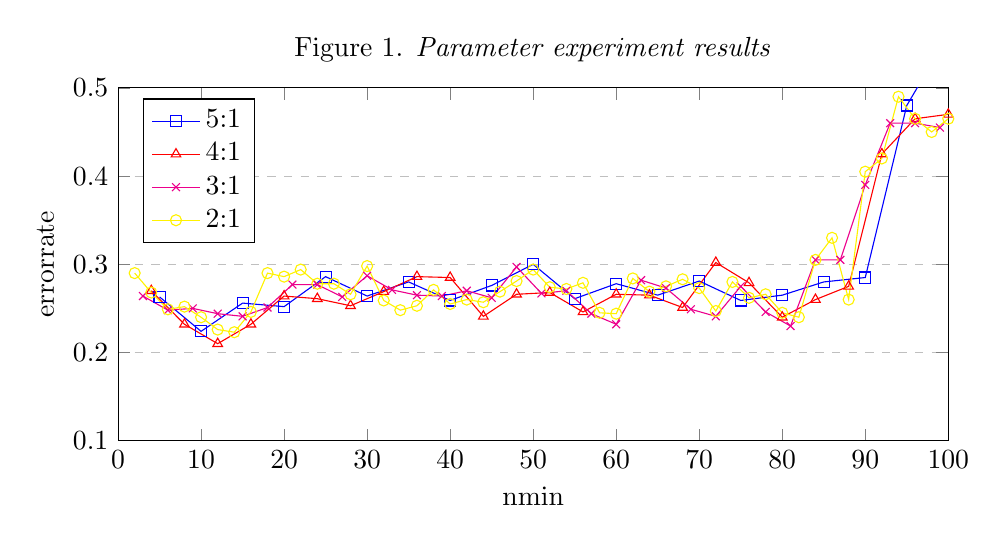
\begin{tikzpicture}
        \begin{axis}[
            title={Figure 1. \textit{Parameter experiment results}},
            xlabel={nmin},
            ylabel={errorrate},
            xmin=0, xmax=100,
            ymin=0.1, ymax=0.5,
            width=1\textwidth,
            height=0.5\textwidth,
            legend pos=north west,
            ymajorgrids=true,
            grid style=dashed
        ]
         
        \addplot[color=blue,mark=square,]
            coordinates {
                ( 5.000000,0.263000)(10.000000,0.224000)(15.000000,0.256000)(20.000000,0.252000)(25.00000,0.28600)(30.000000,0.264000)(35.000000,0.280000)(40.00000,0.25900)(45.000000,0.276000)(50.00000,0.30000)(55.0000000,0.2610000)(60.0000000,0.2780000)(65.0000000,0.2650000)(70.0000000,0.2810000)(75.0000000,0.2590000)(80.0000000,0.2650000)(85.0000000,0.2800000)(90.0000000,0.2850000)(95.0000000,0.4800000)(100.0000000,0.5600000)

            };
            \addlegendentry{5:1}

        \addplot[color=red,mark=triangle,]
            coordinates {
                ( 4.000000,0.270000)( 8.000000,0.232000)(12.000000,0.210000)(16.000000,0.232000)(20.00000,0.26400)(24.000000,0.261000)(28.000000,0.253000)(32.000000,0.269000)(36.000000,0.286000)(40.000000,0.285000)(44.000000,0.241000)(48.0000000,0.2660000)(52.0000000,0.2680000)(56.0000000,0.2460000)(60.000000,0.266000)(64.0000000,0.2650000)(68.0000000,0.2510000)(72.0000000,0.3020000)(76.0000000,0.2790000)(80.0000000,0.2400000)(84.0000000,0.2600000)(88.0000000,0.2750000)(92.0000000,0.4250000)(96.0000000,0.4650000)(100.0000000,0.4700000)
            };
            \addlegendentry{4:1}
            
            \addplot[color=magenta,mark=x,]
                coordinates {
                    ( 3.000000,0.264000)( 6.000000,0.248000)( 9.000000,0.250000)(12.000000,0.244000)(15.000000,0.241000)(18.000000,0.251000)(21.000000,0.277000)(24.000000,0.277000)(27.000000,0.263000)(30.000000,0.287000)(33.000000,0.271000)(36.000000,0.265000)(39.000000,0.264000)(42.000000,0.270000)(45.0000000,0.2620000)(48.0000000,0.2970000)(51.0000000,0.2670000)(54.0000000,0.2700000)(57.0000000,0.2440000)(60.0000000,0.2320000)(63.0000000,0.2820000)(66.0000000,0.2730000)(69.0000000,0.2490000)(72.000000,0.241000)(75.0000000,0.2750000)(78.0000000,0.2460000)(81.000000,0.230000)(84.0000000,0.3050000)(87.0000000,0.3050000)(90.0000000,0.3900000)(93.0000000,0.4600000)(96.000000,0.460000)(99.0000000,0.4550000)
                };   
            \addlegendentry{3:1}

            \addplot[color=yellow,mark=o,]
                coordinates{
                  (2.000000,  0.290000)  (4.000000,  0.268000)  (6.000000,  0.249000)  (8.000000,  0.252000) (10.000000,  0.240000) (12.000000,  0.226000) (14.000000,  0.223000) (16.000000,  0.246000) (18.000000,  0.290000) (20.00000,  0.28600) (22.000000,  0.294000) (24.000000,  0.278000) (26.000000,  0.278000) (28.000000,  0.266000) (30.000000,  0.298000) (32.000000,  0.259000) (34.000000,  0.248000) (36.000000,  0.253000) (38.000000,  0.271000) (40.000000,  0.255000) (42.000000,  0.260000) (44.000000,  0.257000) (46.0000000,  0.2690000) (48.0000000,  0.2810000) (50.0000000,  0.2940000) (52.0000000,  0.2740000) (54.0000000,  0.2720000) (56.0000000,  0.2790000) (58.000000,  0.245000) (60.0000000,  0.2440000) (62.0000000,  0.2840000) (64.0000000,  0.2690000) (66.0000000,  0.2750000) (68.0000000,  0.2830000) (70.0000000,  0.2730000) (72.0000000,  0.2470000) (74.000000,  0.280000) (76.0000000,  0.2620000) (78.0000000,  0.2660000) (80.0000000,  0.2450000) (82.0000000,  0.2400000) (84.0000000,  0.3050000) (86.0000000,  0.3300000) (88.0000000,  0.2600000) (90.0000000,  0.4050000) (92.0000000,  0.4200000) (94.0000000,  0.4900000) (96.0000000,  0.4650000) (98.000000,  0.450000) (100.0000000,   0.4650000)
                };
            \addlegendentry{2:1}

        \end{axis}
    \end{tikzpicture}

    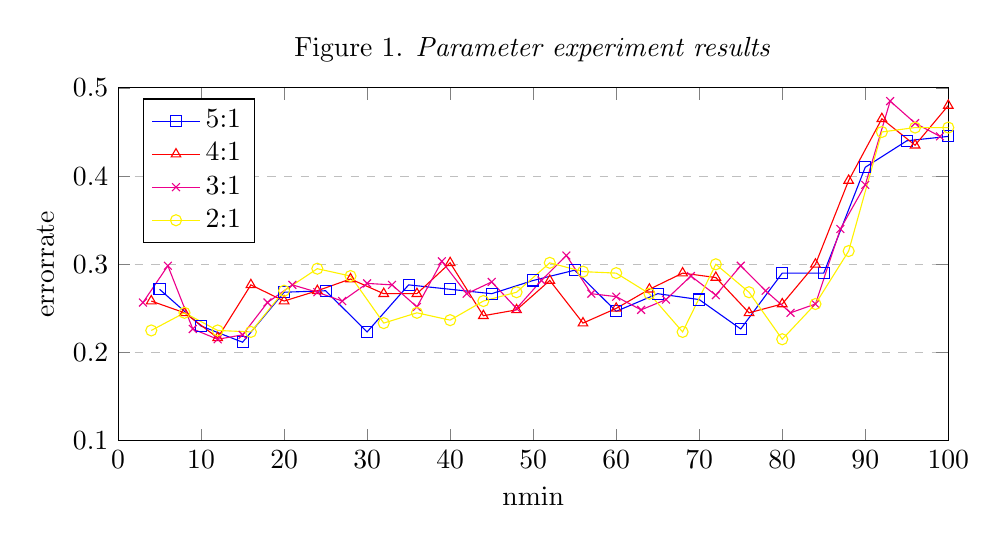
\begin{tikzpicture}
        \begin{axis}[
            title={Figure 1. \textit{Parameter experiment results}},
            xlabel={nmin},
            ylabel={errorrate},
            xmin=0, xmax=100,
            ymin=0.1, ymax=0.5,
            width=1\textwidth,
            height=0.5\textwidth,
            legend pos=north west,
            ymajorgrids=true,
            grid style=dashed
        ]
         
        \addplot[color=blue,mark=square,]
            coordinates {
                (5.0000000,0.2716667)(10.000000,0.230000)(15.0000000,0.2116667)(20.0000000,0.2683333)(25.000000,0.270000)(30.0000000,0.2233333)(35.0000000,0.2766667)(40.0000000,0.2716667)(45.0000000,0.2666667)(50.0000000,0.2816667)(55.0000000,0.2933333)(60.0000000,0.2466667)(65.0000000,0.2666667)(70.0000000,0.2600000)(75.0000000,0.2266667)(80.0000000,0.2900000)(85.0000000,0.2900000)(90.0000000,0.4100000)(95.0000000,0.4400000)(100.000000,0.445000)

            };
            \addlegendentry{5:1}

        \addplot[color=red,mark=triangle,]
            coordinates {
                (4.0000000,0.2583333)(8.000000,0.245000)(12.0000000,0.2166667)(16.0000000,0.2766667)(20.0000000,0.2583333)(24.000000,0.270000)(28.0000000,0.2833333)(32.0000000,0.2666667)(36.0000000,0.2666667)(40.0000000,0.3016667)(44.0000000,0.2416667)(48.0000000,0.2483333)(52.0000000,0.2816667)(56.0000000,0.2333333)(60.000000,0.250000)(64.0000000,0.2716667)(68.0000000,0.2900000)(72.0000000,0.2850000)(76.0000000,0.2450000)(80.0000000,0.2550000)(84.0000000,0.3000000)(88.000000,0.395000)(92.0000000,0.4650000)(96.000000,0.435000)(100.0000000,0.4800000)
            };
            \addlegendentry{4:1}
            
            \addplot[color=magenta,mark=x,]
                coordinates {
                    (3.0000000,0.2566667)(6.0000000,0.2983333)(9.0000000,0.2266667)(12.000000,0.215000)(15.000000,0.220000)(18.0000000,0.2566667)(21.0000000,0.2766667)(24.0000000,0.2683333)(27.0000000,0.2583333)(30.0000000,0.2783333)(33.0000000,0.2766667)(36.0000000,0.2516667)(39.0000000,0.3033333)(42.0000000,0.2666667)(45.0000000,0.2800000)(48.000000,0.250000)(51.0000000,0.2816667)(54.0000000,0.3100000)(57.0000000,0.2666667)(60.0000000,0.2633333)(63.0000000,0.2483333)(66.0000000,0.2600000)(69.0000000,0.2866667)(72.0000000,0.2650000)(75.0000000,0.2983333)(78.0000000,0.2700000)(81.0000000,0.2450000)(84.0000000,0.2550000)(87.0000000,0.3400000)(90.0000000,0.3900000)(93.0000000,0.4850000)(96.0000000,0.4600000)(99.0000000,0.4450000)
                };   
            \addlegendentry{3:1}

            \addplot[color=yellow,mark=o,]
                coordinates{
                    (4.000000,0.225000)(8.000000,0.245000)(12.000000,0.225000)(16.0000000,0.2233333)(20.000000,0.270000)(24.00000,0.29500)(28.0000000,            0.2866667)(32.0000000,0.2333333)(36.000000,0.245000)(40.0000000,0.2366667)(44.0000000,0.2583333)(48.0000000,0.2683333)(52.0000000,0.3016667)(56.0000000,0.2916667)(60.0000000,0.2900000)(64.0000000,0.2666667)(68.0000000,0.2233333)(72.0000000,0.3000000)(76.0000000,0.2683333)(80.000000,0.215000)(84.0000000,0.2550000)(88.0000000,0.3150000)(92.0000000,0.4500000)(96.0000000,0.4550000)(100.0000000,0.4550000)
                };
            \addlegendentry{2:1}

        \end{axis}
    \end{tikzpicture}

\tikzset{
  treenode/.style = {align=center, inner sep=0pt, text centered,
    font=\sffamily}
}

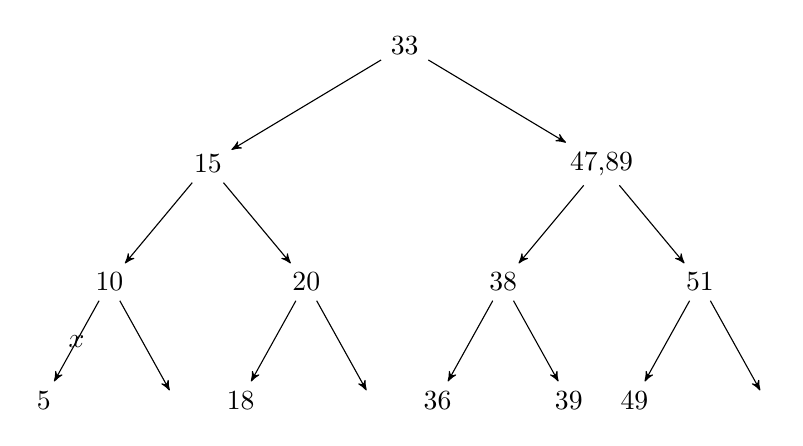
\begin{tikzpicture}[->,>=stealth',level/.style={sibling distance = 5cm/#1,
  level distance = 1.5cm}] 
\node {33}
    child{ node {15} 
            child{ node {10} 
                child{ node {5} edge from parent node[]
                         {$x$}} %for a named pointer
                            child{ node {}}
            }
            child{ node {20}
                            child{ node {18}}
                            child{ node {}}
            }                            
    }
    child{ node {47,89}
            child{ node {38} 
                            child{ node {36}}
                            child{ node {39}}
            }
            child{ node {51}
                            child{ node {49}}
                            child{ node {}}
            }
        }
; 
\end{tikzpicture}
\end{document}

\section{Results}





\end{document}